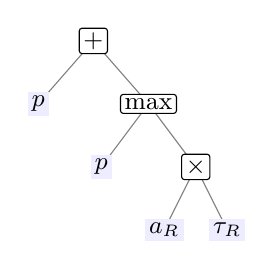
\begin{tikzpicture}[x=8mm,y=8mm,every node/.style={font=\small,inner sep=1.5pt}]
\draw[gray] (2.5,-2) -- (2,-3);
\draw[gray] (2.5,-2) -- (3,-3);
\draw[gray] (1.75,-1) -- (1,-2);
\draw[gray] (1.75,-1) -- (2.5,-2);
\draw[gray] (0.875,0) -- (0,-1);
\draw[gray] (0.875,0) -- (1.75,-1);
\node[fill=blue!7] at (0,-1) {$p$};
\node[fill=blue!7] at (1,-2) {$p$};
\node[fill=blue!7] at (2,-3) {$a_R$};
\node[fill=blue!7] at (3,-3) {$\tau_R$};
\node[draw,rounded corners=1pt,fill=white] at (2.5,-2) {$\times$};
\node[draw,rounded corners=1pt,fill=white] at (1.75,-1) {$\max$};
\node[draw,rounded corners=1pt,fill=white] at (0.875,0) {$+$};
\end{tikzpicture}
